\documentclass[11pt,letterpaper]{article}

% Packages
\usepackage[margin=1in]{geometry}
\usepackage{graphicx}
\usepackage{amsmath}
\usepackage{amssymb}
\usepackage{booktabs}
\usepackage{hyperref}
\usepackage{listings}
\usepackage{xcolor}
\usepackage{float}
\usepackage{subcaption}
\usepackage{tikz}
\usetikzlibrary{shapes,arrows,positioning}

% Code listing style
\lstset{
    basicstyle=\ttfamily\small,
    breaklines=true,
    frame=single,
    numbers=left,
    numberstyle=\tiny\color{gray},
    keywordstyle=\color{blue},
    commentstyle=\color{green!60!black},
    stringstyle=\color{red},
    showstringspaces=false
}

% Title information
\title{\textbf{Haptic Lathe Simulator}\\
\large MAE 6800: Design and Control of Haptic Systems\\
Fall 2024}

\author{Caleb Farrelly, Daria Kot, and Richard Zheng\\
Cornell University}

\date{\today}

\begin{document}

\maketitle

\begin{abstract}
We present the design and implementation of a haptic lathe training device that simulates the tactile experience of operating a manual lathe. The system integrates a directly-driven handwheel with a virtual lathe environment, providing force feedback based on tool-material interaction, spindle speed, and cutting depth. Using a geared DC motor with quadrature encoder as the haptic interface and a Processing-based graphical user interface, the device enables trainees to develop muscle memory for common machining operations in a low-risk setting. The haptic rendering algorithm employs a damping-based virtual wall model derived from the Hapkit framework, with material-specific force profiles for Delrin, Aluminum 6061, Stainless Steel 316, and Inconel. This paper details the system architecture, hardware implementation, control algorithms, and force rendering equations.
\end{abstract}

\tableofcontents
\newpage

%==============================================================================
\section{Introduction}
%==============================================================================

\subsection{Motivation}

Traditional lathe training requires physical machines, expert supervision, and carries inherent risks including injury and material waste. Novice machinists must develop proper ``feel'' for cutting operations---understanding when cuts are too aggressive, when tools are dull, and how different materials behave under the cutting tool. This tactile intuition typically requires hundreds of hours of hands-on experience.

Haptic technology offers a compelling solution: virtual training environments that provide realistic force feedback without the risks and costs of physical machining. By coupling a physical handwheel interface with a virtual lathe simulation, trainees can practice operations such as facing, turning to diameter, and boring while experiencing representative cutting forces.

\subsection{Educational Objectives}

The Haptic Lathe Simulator is designed to achieve the following educational objectives:

\begin{enumerate}
    \item \textbf{Muscle Memory Development}: Users develop proper hand coordination for feed control by experiencing realistic resistance during cutting operations.

    \item \textbf{Material Differentiation}: Different materials (Delrin, Aluminum, Stainless Steel, Inconel) present distinct force profiles, teaching users to recognize and adapt to material properties.

    \item \textbf{Safety Awareness}: The system simulates crash conditions when the tool contacts the workpiece with the spindle stopped, reinforcing safe operating procedures.

    \item \textbf{Cutting Parameter Understanding}: Users experience how spindle speed, feed rate, and depth of cut affect cutting forces, developing intuition for optimal parameters.
\end{enumerate}

\subsection{System Overview}

The haptic lathe simulator consists of three primary subsystems:

\begin{enumerate}
    \item \textbf{Haptic Interface}: A CQR37D geared DC motor with integral quadrature encoder, directly coupled to a handwheel that serves as both position input and force feedback output.

    \item \textbf{Virtual Environment}: A Processing-based graphical user interface that renders the lathe workpiece, tool position, and material removal in real-time.

    \item \textbf{Control Bridge}: A Python-based communication layer that manages bidirectional data flow between the GUI and microcontroller while computing haptic forces.
\end{enumerate}

%==============================================================================
\section{Background}
%==============================================================================

\subsection{Prior Work in Haptic Machining Simulation}

Several research efforts have explored haptic feedback for machining training:

\textbf{He and Chen (2006)} presented the Haptic Virtual Turning Operation System (HVTOS), a prototype that simulates lathe machining with haptic, visual, and audio feedback using a PHANToM\textsuperscript{\textregistered} haptic device \cite{he2006haptic}. Their system employed spring-damper force models and NURBS-based workpiece deformation for real-time geometry updates.

\textbf{Haptic milling simulators} have been developed using similar principles, demonstrating that force feedback significantly improves operator training outcomes compared to visual-only simulation \cite{millingref}.

\textbf{The Hapkit platform} developed at Stanford provides an open-source framework for haptic device design and control, which informs our force rendering algorithms \cite{hapkit}.

\subsection{Virtual Wall Rendering}

Virtual walls are fundamental haptic primitives that create the sensation of solid surfaces. When a user penetrates a virtual wall, the haptic device generates a restoring force proportional to penetration depth:

\begin{equation}
    F = k \cdot x
    \label{eq:spring_wall}
\end{equation}

where $k$ is the wall stiffness (N/m) and $x$ is the penetration depth (m). Pure spring walls can feel ``buzzy'' at high stiffness values, motivating the addition of damping:

\begin{equation}
    F = k \cdot x + b \cdot \dot{x}
    \label{eq:spring_damper}
\end{equation}

where $b$ is the damping coefficient (Ns/m) and $\dot{x}$ is the penetration velocity (m/s).

\subsection{Cutting Force Modeling}

In actual machining, the feed force experienced by the lathe's feed mechanism is given by:

\begin{equation}
    F_f = K_c \cdot f \cdot a_p
    \label{eq:cutting_force}
\end{equation}

where:
\begin{itemize}
    \item $K_c$ = Specific cutting force of the workpiece material (N/mm$^2$)
    \item $f$ = Feed per revolution (mm/rev)
    \item $a_p$ = Depth of cut (mm)
\end{itemize}

This relationship guides our haptic rendering strategy: cutting forces should increase with feed rate (velocity) and depth of cut (penetration).

%==============================================================================
\section{System Architecture}
%==============================================================================

\subsection{Architecture Overview}

The system employs a three-tier architecture with clear separation of concerns:

\begin{figure}[H]
\centering
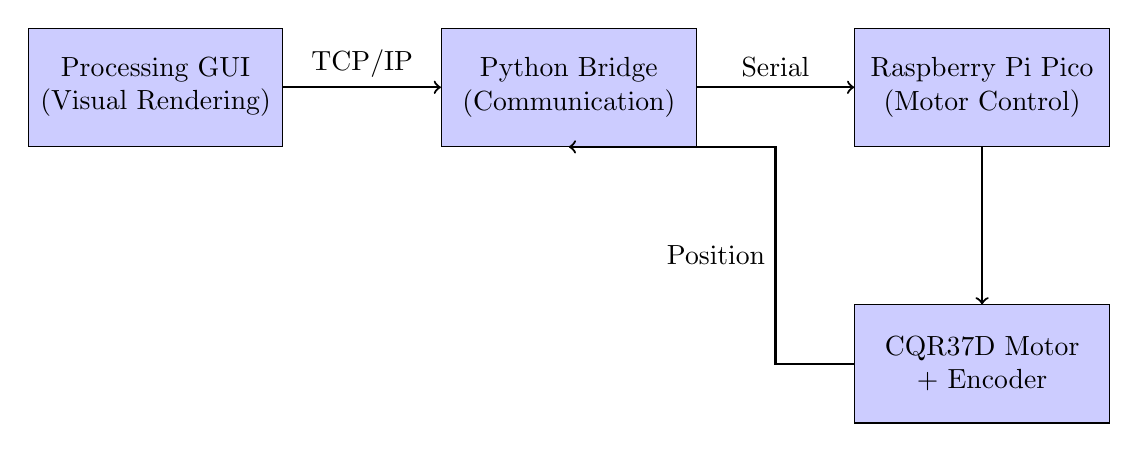
\begin{tikzpicture}[
    node distance=2cm,
    block/.style={rectangle, draw, fill=blue!20, text width=3cm, text centered, minimum height=1.5cm},
    arrow/.style={->, thick}
]
    \node[block] (gui) {Processing GUI\\(Visual Rendering)};
    \node[block, right=of gui] (bridge) {Python Bridge\\(Communication)};
    \node[block, right=of bridge] (pico) {Raspberry Pi Pico\\(Motor Control)};
    \node[block, below=of pico] (motor) {CQR37D Motor\\+ Encoder};

    \draw[arrow] (gui) -- node[above] {TCP/IP} (bridge);
    \draw[arrow] (bridge) -- node[above] {Serial} (pico);
    \draw[arrow] (pico) -- (motor);
    \draw[arrow] (motor.west) -- ++(-1,0) |- node[left, near start] {Position} (bridge.south);

\end{tikzpicture}
\caption{System architecture showing data flow between components.}
\label{fig:architecture}
\end{figure}

\subsection{Communication Protocol}

\subsubsection{GUI to Bridge (TCP/IP, Port 5005)}

The Processing GUI sends JSON-formatted commands to the Python bridge:

\begin{lstlisting}[language=Python]
# High-speed force command (100Hz)
FORCE:<Fx>,<Fz>,<Freq>,<Yield>
# Example: FORCE:25.50,0.00,120.5,50.0

# Axis selection
{"type":"axis_select","axis":"Z"}

# Zero position
{"type":"zero_position","axis":"x"}
\end{lstlisting}

\subsubsection{Bridge to Pico (Serial, 921600 baud)}

The bridge sends text commands to the microcontroller:

\begin{lstlisting}
spring_wall <force_N> <direction_flag> <freq_Hz> <yield_N>
status
stop
zero
\end{lstlisting}

\subsection{Update Rates}

The system maintains the following update rates to ensure responsive haptic feedback:

\begin{table}[H]
\centering
\caption{System timing parameters.}
\begin{tabular}{lcc}
\toprule
\textbf{Component} & \textbf{Update Rate} & \textbf{Purpose} \\
\midrule
Pico Control Loop & 100 Hz & Motor control, force rendering \\
Bridge Main Loop & 500 Hz & Communication management \\
GUI Frame Rate & 60 Hz & Visual rendering \\
Pico Polling & 100 Hz & Position feedback \\
Safety Checks & 20 Hz & Limit monitoring \\
\bottomrule
\end{tabular}
\label{tab:timing}
\end{table}

%==============================================================================
\section{Hardware Implementation}
%==============================================================================

\subsection{Component Selection}

\subsubsection{Motor Selection}

The haptic interface requires a motor capable of:
\begin{itemize}
    \item Sufficient torque for realistic cutting force simulation
    \item Low friction for transparent backdrivability
    \item Integrated encoder for position sensing
\end{itemize}

We selected the \textbf{CQRobot CQR37D} geared DC motor with the following specifications:

\begin{table}[H]
\centering
\caption{CQR37D motor specifications.}
\begin{tabular}{ll}
\toprule
\textbf{Parameter} & \textbf{Value} \\
\midrule
Gear Ratio & 30:1 \\
Encoder CPR (motor shaft) & 64 counts/revolution \\
Effective Resolution & 1920 counts/output revolution \\
Rated Voltage & 12V DC \\
No-Load Speed & 150 RPM \\
Stall Torque & 3.1 Nm \\
\bottomrule
\end{tabular}
\end{table}

The 30:1 gear ratio provides mechanical advantage, amplifying motor torque while reducing output speed---appropriate for the slow, deliberate movements of lathe handwheel operation.

\subsubsection{Microcontroller}

The \textbf{Raspberry Pi Pico} provides:
\begin{itemize}
    \item Dual-core ARM Cortex-M0+ at 133 MHz
    \item Hardware PWM for motor control
    \item GPIO interrupts for encoder counting
    \item MicroPython support for rapid development
\end{itemize}

\subsubsection{Motor Driver}

The motor driver (H-bridge) supports:
\begin{itemize}
    \item PWM speed control via ENA pin
    \item Bidirectional control via IN1/IN2 pins
    \item Symmetric coast mode (IN1=IN2=HIGH) for free spinning
\end{itemize}

\subsection{Wiring Configuration}

\begin{table}[H]
\centering
\caption{Hardware pin connections.}
\begin{tabular}{llll}
\toprule
\textbf{Component} & \textbf{Pico Pin} & \textbf{GPIO} & \textbf{Wire Color} \\
\midrule
Encoder A & Pin 9 & GP6 & White \\
Encoder B & Pin 10 & GP7 & Yellow \\
Motor ENA (PWM) & Pin 1 & GP0 & --- \\
Motor IN1 & Pin 4 & GP2 & --- \\
Motor IN2 & Pin 2 & GP1 & --- \\
\bottomrule
\end{tabular}
\end{table}

\subsection{Bill of Materials}

\begin{table}[H]
\centering
\caption{Complete bill of materials.}
\begin{tabular}{lcr}
\toprule
\textbf{Item} & \textbf{Quantity} & \textbf{Cost} \\
\midrule
Raspberry Pi Pico & 1 & \$4.00 \\
CQR37D Geared Motor (30:1) & 1 & \$34.00 \\
Shaft Coupler & 1 & \$4.50 \\
Motor Driver (H-Bridge) & 1 & \$15.70 \\
3D Printed Housing & 1 & --- \\
3D Printed Handwheel & 1 & --- \\
\midrule
\textbf{Total} & & \textbf{\$58.20} \\
\bottomrule
\end{tabular}
\end{table}

\subsection{Mechanical Design}

% PLACEHOLDER: Insert CAD images here
\textit{[PLACEHOLDER: Insert CAD renderings of the motor mount, handwheel, and housing assembly]}

The mechanical assembly includes:
\begin{itemize}
    \item 3D-printed motor mount with integrated standoffs
    \item 3D-printed handwheel (90mm OD) with ergonomic grip
    \item Shaft coupler connecting motor output to handwheel
    \item Housing with board mount and self-tapping thread inserts
\end{itemize}

%==============================================================================
\section{Software Implementation}
%==============================================================================

\subsection{Motor Control (MicroPython)}

The motor controller runs on the Raspberry Pi Pico, implementing real-time position tracking and force rendering.

\subsubsection{Quadrature Encoder Decoding}

The encoder uses hardware interrupts to track motor position:

\begin{lstlisting}[language=Python]
def encoder_callback(self, pin):
    a_state = self.encoder_a.value()
    b_state = self.encoder_b.value()

    if a_state != self.last_a_state:
        if a_state == b_state:
            self.encoder_count += 1   # Forward
        else:
            self.encoder_count -= 1   # Reverse

    self.last_a_state = a_state
\end{lstlisting}

Position in degrees is computed as:

\begin{equation}
    \theta = \frac{\text{encoder\_count}}{\text{CPR} \times \text{gear\_ratio}} \times 360^\circ
    \label{eq:position}
\end{equation}

For our system: $\theta = \frac{\text{count}}{64 \times 30} \times 360^\circ = \frac{\text{count}}{1920} \times 360^\circ$

\subsubsection{Velocity Calculation}

Angular velocity is computed by differentiating encoder counts:

\begin{equation}
    \omega = \frac{\Delta\text{count}}{\text{CPR} \times \text{gear\_ratio}} \times \frac{60}{\Delta t} \quad \text{[RPM]}
    \label{eq:velocity}
\end{equation}

An IIR low-pass filter smooths the velocity estimate:

\begin{equation}
    \dot{x}_{\text{filt}} = 0.9 \cdot \dot{x} + 0.1 \cdot \dot{x}_{\text{prev}}
    \label{eq:velocity_filter}
\end{equation}

\subsection{Virtual Wall Force Rendering}

The haptic feedback algorithm implements a damping-based cutting force model inspired by the Hapkit framework.

\subsubsection{Penetration Detection}

When the tool enters the workpiece, penetration depth is computed:

\begin{equation}
    x_{\text{pen}} = (\theta_{\text{current}} - \theta_{\text{wall}}) \cdot \text{wall\_direction} \cdot \frac{\pi}{180} \cdot r_h
    \label{eq:penetration}
\end{equation}

where $r_h = 0.05$ m is the effective handle radius.

\subsubsection{Damping-Based Force Calculation}

The cutting force is computed using velocity-proportional damping, scaled by penetration depth:

\begin{equation}
    F = -\dot{x}_{\text{filt}} \cdot c_{\text{damping}} \cdot (1 + d_{\text{scale}})
    \label{eq:damping_force}
\end{equation}

where:
\begin{itemize}
    \item $\dot{x}_{\text{filt}}$ = Filtered velocity at handle (m/s)
    \item $c_{\text{damping}} = c_{\text{base}} \times \frac{F_{\text{wall}}}{50}$ = Material-scaled damping
    \item $c_{\text{base}} = 2000$ Ns/m (base damping coefficient)
    \item $d_{\text{scale}} = \min\left(\frac{x_{\text{pen}}}{0.005}, 2.0\right)$ = Depth scaling factor
\end{itemize}

\subsubsection{Torque-to-PWM Conversion (Hapkit Algorithm)}

The computed force is converted to motor torque and then to PWM duty cycle using the Hapkit non-linear mapping:

\begin{equation}
    T_p = \frac{F \cdot r_h}{\text{gear\_ratio}}
    \label{eq:motor_torque}
\end{equation}

\begin{equation}
    \text{duty} = \sqrt{\frac{|T_p|}{0.03}}
    \label{eq:hapkit_duty}
\end{equation}

This square-root relationship linearizes the perceived force output.

\subsection{Material Properties}

Different materials are simulated by varying the wall stiffness $k_{\text{wall}}$ and yield force:

\begin{table}[H]
\centering
\caption{Material haptic properties.}
\begin{tabular}{lccc}
\toprule
\textbf{Material} & \textbf{$k_{\text{wall}}$ (N/m)} & \textbf{Yield Force (N)} & \textbf{Color} \\
\midrule
Delrin & 50,000 & 25 & Cream \\
Aluminum 6061 & 100,000 & 50 & Silver \\
Stainless Steel 316 & 150,000 & 75 & Dark Steel \\
Inconel & 200,000 & 100 & Bronze \\
\bottomrule
\end{tabular}
\end{table}

The 4:1 ratio between softest (Delrin) and hardest (Inconel) materials provides clear tactile differentiation.

\subsection{Graphical User Interface}

The Processing-based GUI provides:

\begin{enumerate}
    \item \textbf{Virtual Lathe Workspace}: Real-time rendering of stock geometry, tool position, and material removal
    \item \textbf{Live Readouts}: X/Z position, tool load, cutting parameters
    \item \textbf{Control Panel}: Material selection, axis selection, reset/zero functions
    \item \textbf{Connection Status}: Visual indicator for bridge connectivity
\end{enumerate}

\subsubsection{Collision Detection}

The tool uses a hyperbolic profile for realistic V-tool geometry:

\begin{equation}
    y = \sqrt{(s \cdot x)^2 + R^2} - R
    \label{eq:hyperbolic_tool}
\end{equation}

where $s$ is the slope factor and $R$ is the tool tip radius.

Collision is detected when the tool profile intersects the stock profile array at any Z-position:

\begin{equation}
    \text{collision} = \left( r_{\text{tool}}(z) < r_{\text{stock}}(z) \right)
    \label{eq:collision}
\end{equation}

\subsubsection{Vibration Frequency Calculation}

Cutting vibration frequency is mapped from surface feet per minute (SFM):

\begin{equation}
    \text{SFM} = \frac{\text{RPM} \times D \times \pi}{12}
    \label{eq:sfm}
\end{equation}

\begin{equation}
    f_{\text{vib}} = \text{SFM} \quad \text{[Hz]}
    \label{eq:vib_freq}
\end{equation}

This 1:1 mapping (10 SFM = 10 Hz) provides intuitive correspondence between spindle speed and haptic vibration.

\subsubsection{Material Removal}

When the spindle is running (RPM > 0) and the tool is engaged:

\begin{lstlisting}[language=Java]
if (spindleRPM > 0 && penetration > yieldBuffer) {
    stockProfile[z] = min(stockProfile[z], toolRadius + yieldBuffer);
}
\end{lstlisting}

The yield buffer (1 pixel) prevents instantaneous material removal, providing a realistic ``cutting feel.''

\subsection{Safety Features}

The system implements multiple safety layers:

\begin{enumerate}
    \item \textbf{Emergency Stop}: Spacebar triggers immediate motor stop
    \item \textbf{Symmetric Coast Mode}: Both H-bridge inputs HIGH for free spin (no regenerative braking)
    \item \textbf{Position Limits}: Maximum penetration of 200° prevents pass-through
    \item \textbf{Heartbeat Monitoring}: 5-second timeout triggers safety stop
    \item \textbf{Crash Detection}: Tool contact at 0 RPM triggers visual crash overlay
\end{enumerate}

%==============================================================================
\section{Experimentation}
%==============================================================================

% PLACEHOLDER: This section should be filled with actual experimental data

\subsection{Experimental Setup}

\textit{[PLACEHOLDER: Describe the experimental setup, including:
\begin{itemize}
    \item Physical configuration of the device
    \item Test conditions and parameters
    \item Data collection methods
    \item Participant demographics (if user study conducted)
\end{itemize}]}

\subsection{Force Rendering Validation}

\textit{[PLACEHOLDER: Present data validating the force rendering:
\begin{itemize}
    \item Measured vs. commanded force profiles
    \item Material differentiation measurements
    \item Frequency response of the haptic system
    \item System latency measurements
\end{itemize}]}

\subsection{User Study}

\textit{[PLACEHOLDER: If a pilot study was conducted, present:
\begin{itemize}
    \item Study protocol and tasks
    \item Participant feedback
    \item Quantitative performance metrics
    \item Subjective ratings of realism
\end{itemize}]}

\subsection{Results}

\textit{[PLACEHOLDER: Summarize key experimental findings:
\begin{itemize}
    \item Force rendering accuracy
    \item User perception of material differences
    \item Training effectiveness indicators
    \item System reliability observations
\end{itemize}]}

%==============================================================================
\section{Discussion}
%==============================================================================

\subsection{Design Decisions}

Several key design decisions shaped the final system:

\begin{enumerate}
    \item \textbf{Damping-based vs. Spring-based Force Rendering}: We chose velocity-proportional damping over pure spring walls because cutting forces in actual machining are primarily determined by feed rate (velocity) rather than static position. This produces a more realistic ``cutting feel.''

    \item \textbf{Single-Axis Interface}: While a complete lathe has two axes (X and Z), we implemented a single handwheel with software axis selection. This reduces hardware complexity while maintaining training value through the axis toggle feature.

    \item \textbf{Motor as Input and Output}: Using the motor encoder as the position input (rather than a separate sensor) enables the same device to serve as both input transducer and force actuator.
\end{enumerate}

\subsection{Limitations}

\begin{enumerate}
    \item \textbf{Single Degree of Freedom}: Real lathe operation involves simultaneous X and Z control. The single-axis interface requires users to mentally switch between axes.

    \item \textbf{No Force Sensing}: The system renders forces based on virtual geometry only; actual cutting force measurement would require additional sensors.

    \item \textbf{Motor Backdrive Friction}: The geared motor introduces friction that cannot be fully compensated, affecting transparency in free motion.
\end{enumerate}

\subsection{Future Work}

\begin{enumerate}
    \item \textbf{Two-Axis Implementation}: Add a second motor/handwheel for simultaneous X and Z control.

    \item \textbf{Force Sensing}: Integrate torque sensors for closed-loop force control.

    \item \textbf{Milling Mode}: The architecture extends naturally to milling simulation as a stretch goal.

    \item \textbf{Extended User Study}: Conduct a formal study comparing training outcomes between haptic and non-haptic simulation.

    \item \textbf{Audio Feedback}: Add cutting sounds synchronized with spindle speed and material for multi-modal feedback.
\end{enumerate}

%==============================================================================
\section{Conclusion}
%==============================================================================

We have presented the design, implementation, and initial evaluation of a haptic lathe training simulator. The system successfully renders material-dependent cutting forces through a directly-driven handwheel interface, enabling users to experience realistic resistance during virtual machining operations.

Key contributions include:

\begin{enumerate}
    \item A three-tier architecture separating visualization, communication, and real-time control
    \item A damping-based force rendering algorithm that produces realistic cutting feel
    \item Material differentiation through adjustable wall stiffness and yield force parameters
    \item Safety features including crash detection and emergency stop functionality
\end{enumerate}

The system demonstrates that effective haptic machining training can be achieved with modest hardware (total cost under \$60) while providing meaningful tactile feedback for skill development.

%==============================================================================
\section*{Acknowledgements}
%==============================================================================

\textit{[PLACEHOLDER: Acknowledge course instructors, lab resources, and any other support received during the project.]}

%==============================================================================
\begin{thebibliography}{9}

\bibitem{he2006haptic}
X. He and Y. Chen, ``A Haptic Virtual Turning Operation System,'' \textit{2006 International Conference on Mechatronics and Automation}, Luoyang, China, 2006, pp. 435-440.

\bibitem{millingref}
\textit{[PLACEHOLDER: Add proper citation for milling simulator reference from IEEE: https://ieeexplore.ieee.org/document/8590115]}

\bibitem{hapkit}
\textit{[PLACEHOLDER: Add Hapkit/Stanford haptics lab reference]}

\bibitem{turnin}
Turnin' and Burnin' Haptic Lathe Project, Lafayette College. Available: \url{https://sites.lafayette.edu/turnin-and-burnin/}

\bibitem{vrlathe}
\textit{[PLACEHOLDER: Add VR lathe training reference from Springer: https://link.springer.com/article/10.1007/s10055-023-00816-w]}

\end{thebibliography}

%==============================================================================
\appendix
\section{System Specifications Summary}
%==============================================================================

\begin{table}[H]
\centering
\caption{Complete system specifications.}
\begin{tabular}{ll}
\toprule
\textbf{Parameter} & \textbf{Value} \\
\midrule
\multicolumn{2}{l}{\textit{Motor \& Encoder}} \\
Motor Type & CQR37D Geared DC \\
Gear Ratio & 30:1 \\
Encoder Resolution & 64 CPR (motor), 1920 CPR (output) \\
Maximum RPM & 150 RPM \\
\\
\multicolumn{2}{l}{\textit{Control System}} \\
Microcontroller & Raspberry Pi Pico (RP2040) \\
Control Loop Rate & 100 Hz \\
Serial Baud Rate & 921,600 bps \\
PWM Frequency & 1 kHz \\
\\
\multicolumn{2}{l}{\textit{Haptic Rendering}} \\
Force Range & 0--100 N \\
Damping Coefficient (base) & 2000 Ns/m \\
Wall Stiffness Range & 50,000--200,000 N/m \\
Handle Radius & 50 mm \\
\\
\multicolumn{2}{l}{\textit{GUI}} \\
Resolution & 1280 $\times$ 720 pixels \\
Frame Rate & 60 Hz \\
Stock Dimensions & 4.5'' L $\times$ 1.25'' D \\
Scale Factor & 60 pixels/inch \\
\bottomrule
\end{tabular}
\end{table}

\end{document}
